\section{Auswertung}
Mit dem Aufbau ist es möglich Geschwindigkeiten von über 200 $\nicefrac{km}{h}$ zu erzeugen.

\begin{figure}[ht]
    \centering
    %    \missingfigure{Bild einfügen}
    \includegraphics[width=\textwidth]{images/auswertungSpeedUeb.png}
    \caption{Vergleich unterschiedliche Geschwindigkeiten}
    \label{fig:AuswertungSpeed}
\end{figure}

In \ref{fig:AuswertungSpeed} werden die verschiedenen gemessenen Geschwindigkeit abhängig von der Drehzahl dargestellt.
Erwartet sind folgende Geschwindigkeiten:
\begin{center}
    \begin{tabular}{rr}
        \textbf{RPM}&\textbf{Geschwindigkeit $\left[\nicefrac{km}{h}\right]$}\\ \hline
        100&9.4\\
        500&47.1\\
        750&70.7\\
        1000&94.2\\
        1250&117.8\\
        1500&141.4\\
        1750&164.9\\
        2000&188.5\\
    \end{tabular}
\end{center}
 Die Präzision nimmt mit höherer Geschwindigkeit immer weiter ab, während die Genauigkeit etwa gleich bleibt (vgl. \ref{fig:AuswertungSpeed}, \ref{fig:GenauPraz}). 
% Dieses Verhalten zeigt auch \ref{fig:AuswertungZeitfehler}.

\begin{figure}[ht]
    \centering
    %    \missingfigure{Bild einfügen}
    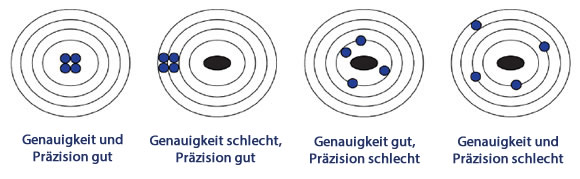
\includegraphics[width=0.7\textwidth]{images/testingtips}
    \caption{Genauigkeit und Präzision}
    \label{fig:GenauPraz}
\end{figure}
\clearpage

In \ref{fig:AuswertungInt} \marg{Vergleich Polling - Interrupt} werden die verschiedene Implementationsmethoden verglichen.\\

Die Daten für Puls LS1 und Puls LS2 wurden durch Polling gewonnen während die restlichen durch Interrupts generiert wurden. Detailliertere Grafiken dazu finden sich in Anhang \ref{app:Auswertung}.
\begin{figure}[ht]
    \centering
%    \missingfigure{Bild einfügen}
    	\includegraphics[width=\textwidth]{images/auswertungInt.png}
    \caption{Vergleich Interrupt und Polling bei 1000 RPM (94.2 $\nicefrac{km}{h}$)}
    \label{fig:AuswertungInt}
\end{figure}


Bei 2000 RPM wurden in beiden Modi jeweils 500 Sample aufgezeichnet und ausgewertet. Dabei wurde eine Präzision von unter 2\% und eine Genauigkeit von unter 5\% erreicht.\\
Die Histogramme aus \ref{fig:Hist} wurde mit Hilfe eines Matlabskripts (Anhang \ref{app:matlab}) erstellt und ausgewertet.\\
% (\href{https://ch.mathworks.com/help/stats/histfit.html}{histfit}). Möglich ist auch eine andere Verteilung. Dies muss genauer untersucht werden.

Berechnung Genauigkeit\marg{Genauigkeit} [\%]:
\[ \frac{|Sollgeschwindigkeit - Mittelwert\;der \; Samples|}{Sollgeschwindigkeit}\cdot 100 \]

Berechnung Präzision \marg{Präzision} [\%]:
\[ \frac{Standardabweichung\;der \; Samples}{Mittelwert\;der \; Samples}\cdot 100 \]

\begin{center}
    \begin{tabular}{lccc}
        \textbf{Mode} & \textbf{Messung} & \textbf{Genauigkeit [\%]} & \textbf{Präzision [\%]} \\ \hline
        Polling       &       LB1        & 4.9                     &  1.9                    \\
        &       LB2        & 3.8                     &  1.6                    \\
        Interrupt     &   LB11 - LB12    & 3.5                     &  1.8                    \\
        &   LB21 - LB22    & 2.4                     &  1.5                    \\
        &   LB11 - LB21    & 3.4                     &  1.2                    \\
        &   LB12 - LB22    & 2.6                     &  1.2 \\
    \end{tabular}
\end{center}

\clearpage

\begin{figure}[H]
    \centering
    %    \missingfigure{Bild einfügen}
    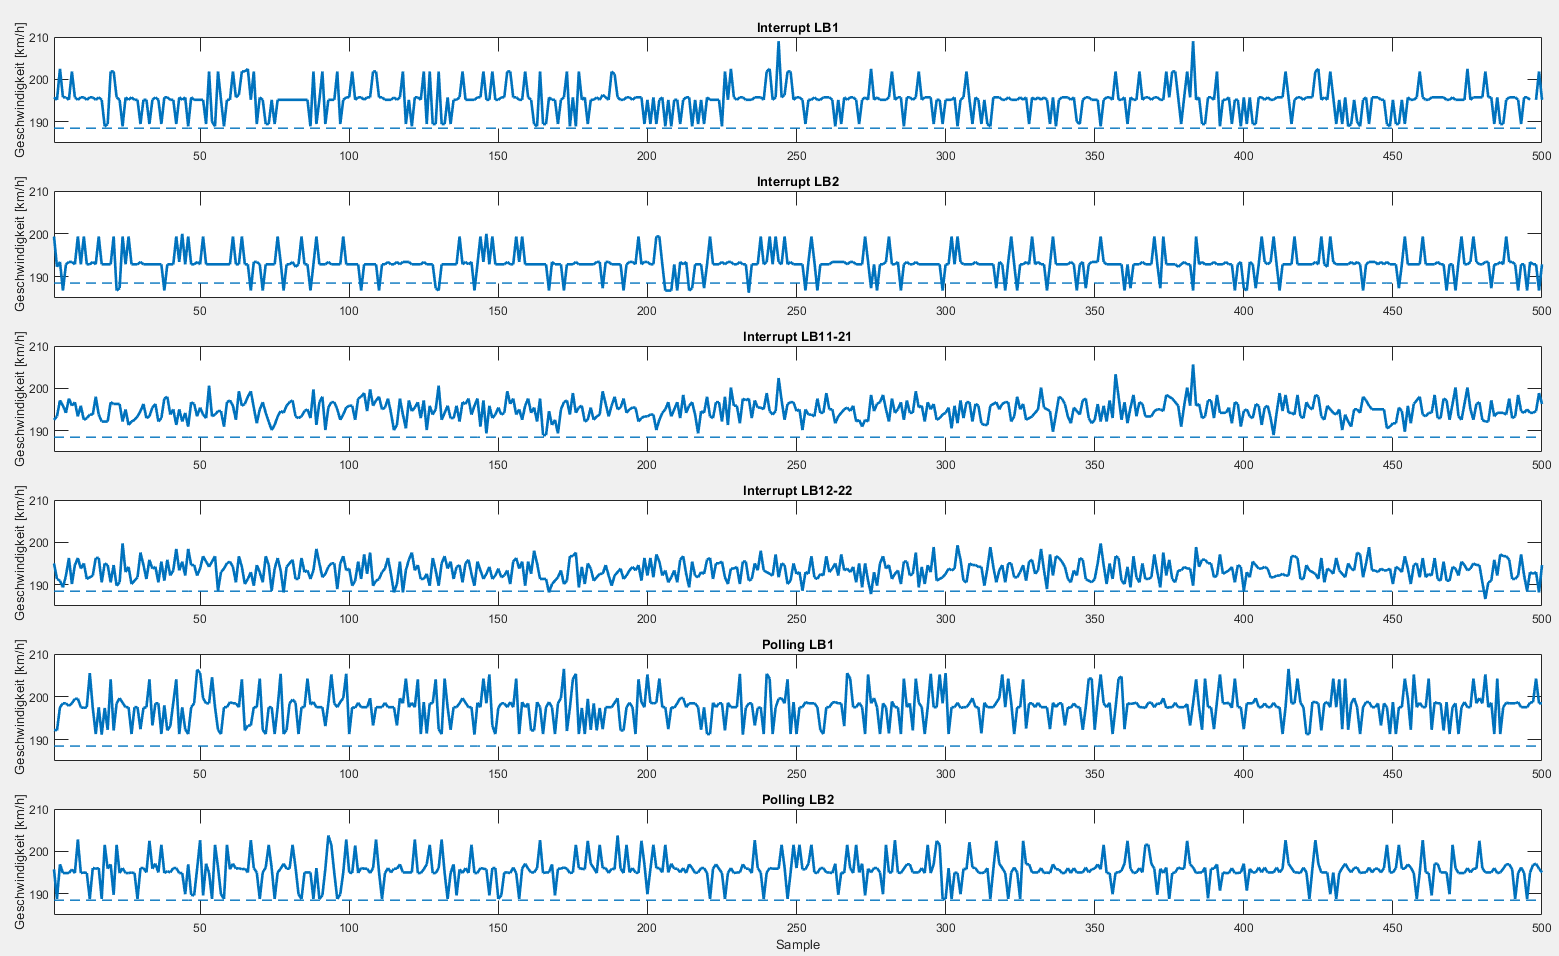
\includegraphics[width=\textwidth]{images/sig2000.png}
    \caption{Gemessene Werte bei 2000 RPM}
    \label{fig:sig2000}
\end{figure}
\begin{figure}[H]
    \centering
    %    \missingfigure{Bild einfügen}
    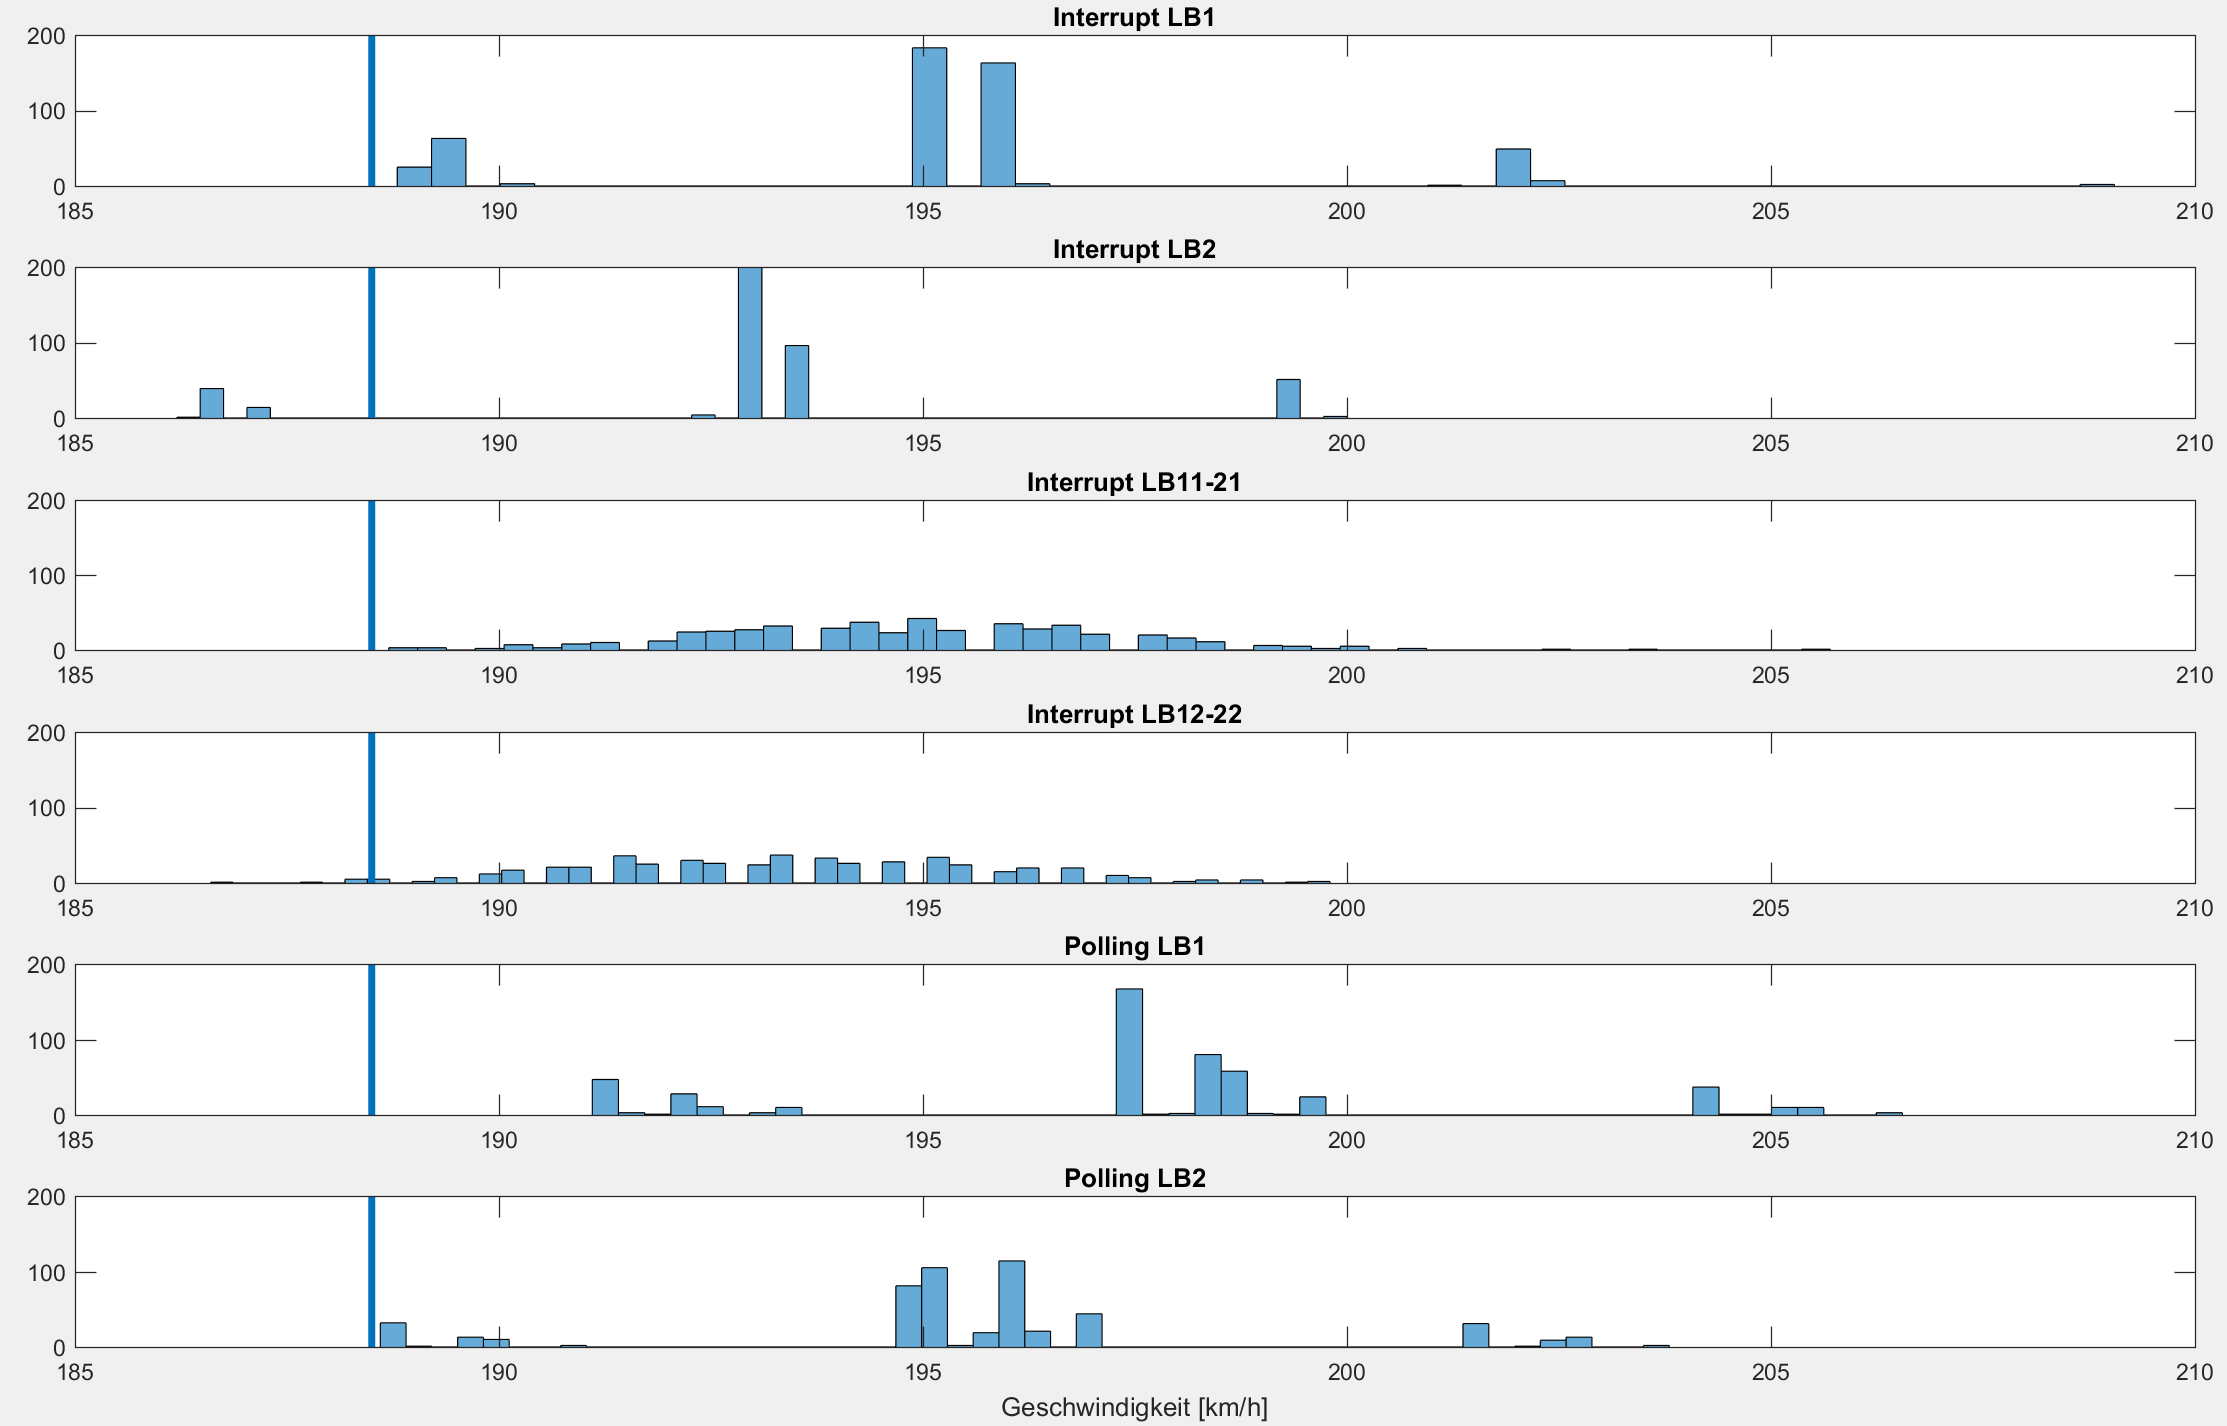
\includegraphics[width=\textwidth]{images/hist2000.png}
    \caption{Histogramm}
    \label{fig:Hist}
\end{figure}

\clearpage
%\begin{figure}[ht]
%    \centering
%    %    \missingfigure{Bild einfügen}
%    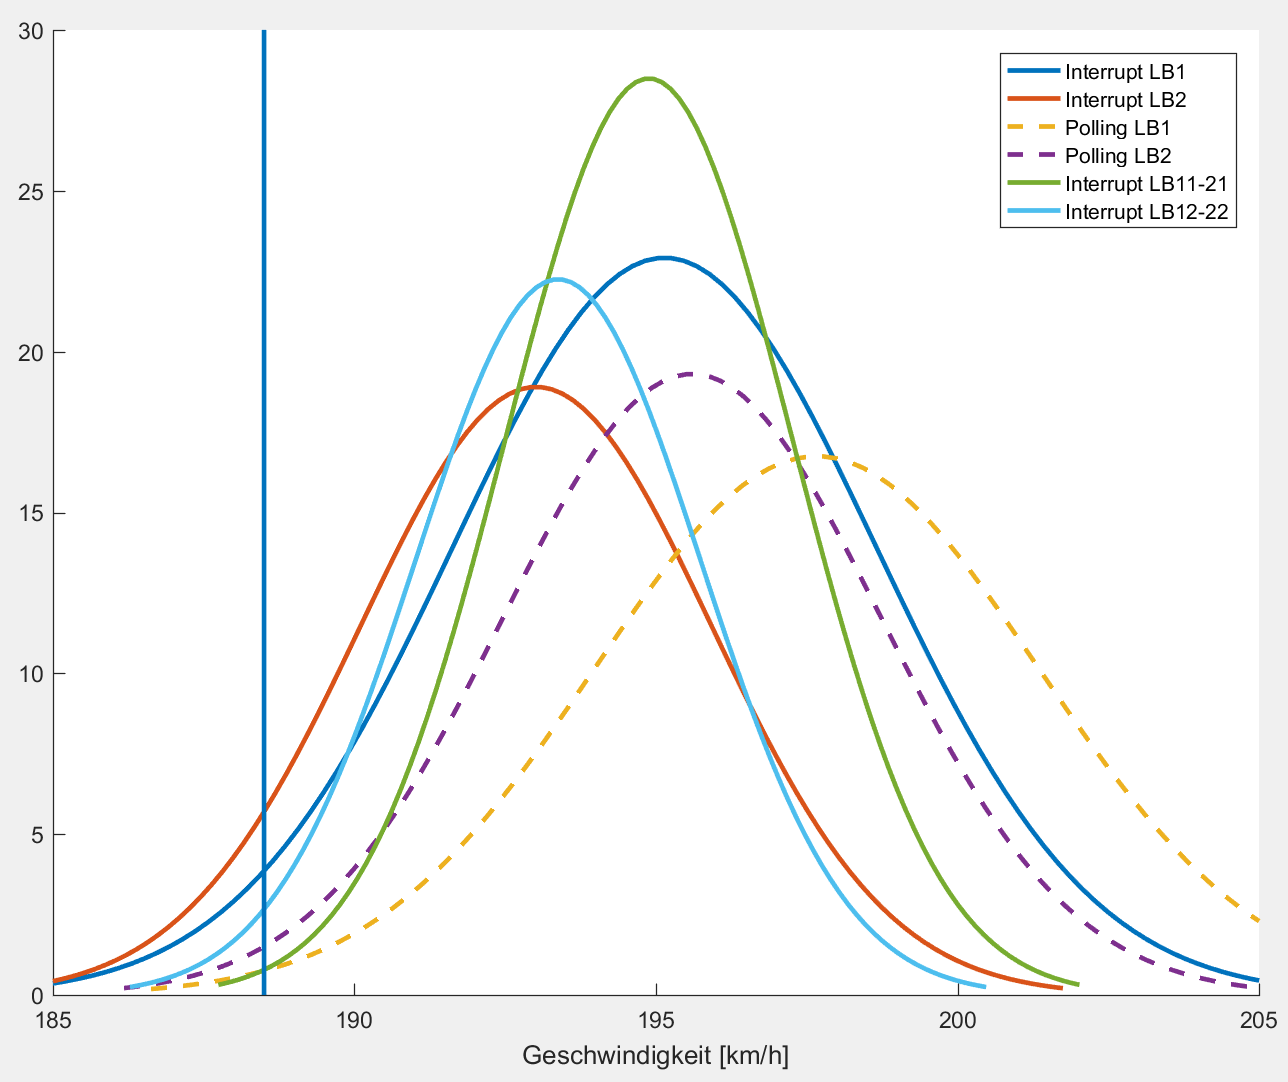
\includegraphics[width=\textwidth]{images/densi.png}
%    \caption{Dichteverteilung}
%    \label{fig:density}
%\end{figure}


%   IntLB1     IntLB2  IntLB1121  IntLB1222   PulsLB1   PulsLB2
%    1.8026    1.5088    1.2213    1.2238    1.8617    1.6057
\clearpage
\subsection{Fehlerquellen}
Die \ref{fig:AuswertungZeitfehler} zeigt den maximalen Geschwindigkeitsfehler wenn mit der maximalen Ansprechzeit der Lichtschranke von 0.5 ms gerechnet wird. Diese Abbildung soll vor allem verdeutlichen, dass Zeitfehler bei hohen Geschwindigkeiten stärker Gewichtet werden.

\begin{figure}[ht]
    \centering
    %    \missingfigure{Bild einfügen}
    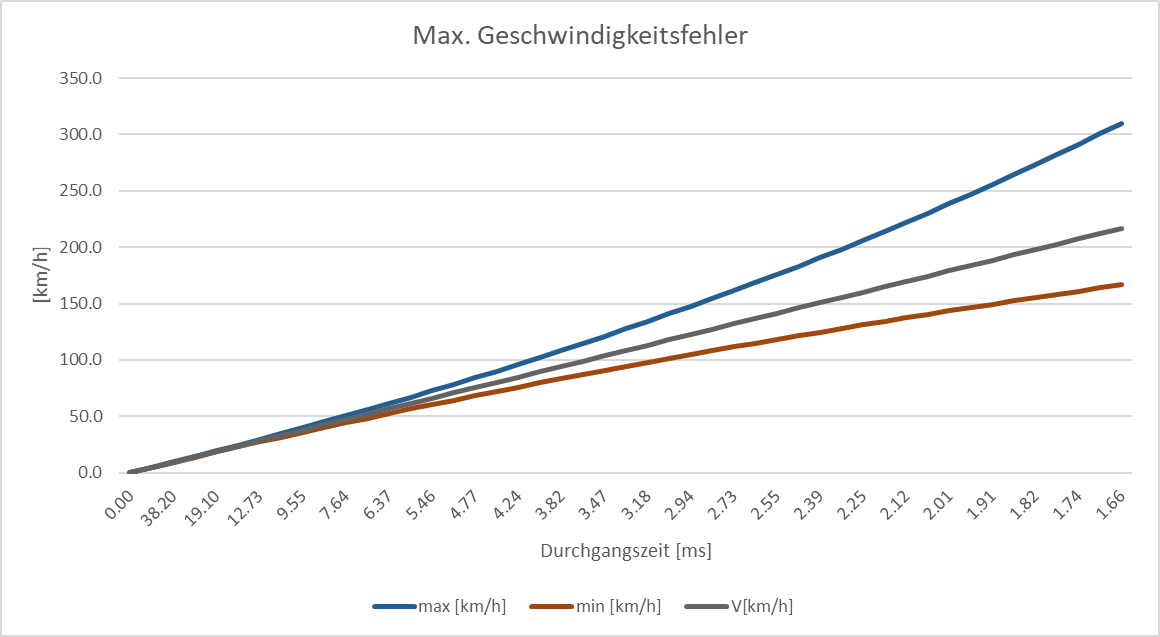
\includegraphics[width=\textwidth]{images/Zeitfehler.png}
    \caption{Max. Geschwindigkeitsfehler maximaler Ansprechverzögerung.}
    \label{fig:AuswertungZeitfehler}
\end{figure}

Die für diesen Versuchsaufbau relevanten \marg{Fehlerquellen}Fehlerquellen sind im Polling-Modus:
\begin{itemize}
    \item Ungenauer Abstand der Lichtschranken zum Drehpunkt des Rotors.
    \item Ungenauigkeit infolge unterschiedlicher Reaktionszeiten der Lichtschranke.
    \begin{itemize}
        \item Wiederholpräzision
        \item Hysterese
    \end{itemize}
    \item Ungenauigkeit infolge Regelabweichung des Motors.
    \item Ungenauigkeit infolge der Reaktionszeit des Arduinos.
\end{itemize}

Beim Interrupt-Modus kommt wegen dem Vergleich zwischen den Lichtschranken noch weitere Ungenauigkeiten dazu:
\begin{itemize}
    \item Ungenauer Abstand der Lichtschranken zueinander.
\end{itemize}
%\null \vspace{0.5\baselineskip}
Die Ungenauigkeit infolge unterschiedlicher Reaktionszeiten der beiden Lichtschranken kann evt. mit dem Aufsetzen einer Schlitzmaske, welche es als Zubehör gibt, auf kosten der Reichweite, noch verbessert werden. Dies würde sich positiv auf die Präzision auswirken. Für eine Verbesserung der Genauigkeit ist vor allem ein geometrisch genauerer Aufbau nötig. \\

Ein weiteres Problem ist, dass auf Grund des rotierenden Aufbaus nicht abschliessend gesagt werden kann, ob alle Durchläufe korrekt detektiert werden. Einzelne Durchläufe könnten nicht detektiert worden sein. Mit diesem Versuchsaufbau ist es jedoch nicht möglich einen einzelnen schnellen Durchgang zu erzeugen.

